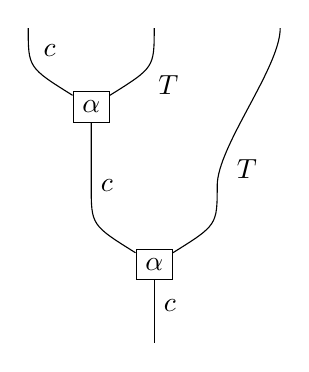
\begin{tikzpicture}[baseline=(current bounding box.center),x=0.8cm]
\path coordinate[] (tikzsd_internal_pos_0_0) at (0.0,0.0);
\path coordinate[] (tikzsd_internal_pos_0_1) at (2.0,0.0);
\path coordinate[] (tikzsd_internal_pos_0_2) at (4.0,0.0);
\path coordinate[] (tikzsd_internal_pos_1_0) at (1.0,-2.0);
\path coordinate[] (tikzsd_internal_pos_1_1) at (3.0,-2.0);
\path coordinate[] (tikzsd_internal_pos_2_0) at (2.0,-4.0);

\path node[,draw,] (tikzsd_internal_nt_node_0_0) at (1.0,-1.0) {$\alpha$};
\path node[,draw,] (tikzsd_internal_nt_node_1_0) at (2.0,-3.0) {$\alpha$};

\path [draw] (tikzsd_internal_pos_0_0) ..controls(0.0,-0.5)..(tikzsd_internal_nt_node_0_0) node[pos=0.5,auto,] {$c$};
\path [draw] (tikzsd_internal_pos_0_1) ..controls(2.0,-0.5)..(tikzsd_internal_nt_node_0_0) node[pos=0.5,auto,] {$T$};
\path [draw] (tikzsd_internal_nt_node_0_0) ..controls(1.0,-1.5)..(tikzsd_internal_pos_1_0) ..controls(1.0,-2.5)..(tikzsd_internal_nt_node_1_0) node[pos=0.0,auto,] {$c$};
\path [draw] (tikzsd_internal_pos_0_2) ..controls(4.0,-0.5)and(3.0,-1.5)..(tikzsd_internal_pos_1_1) node[pos=0.75,auto,] {$T$} ..controls(3.0,-2.5)..(tikzsd_internal_nt_node_1_0);
\path [draw] (tikzsd_internal_nt_node_1_0) ..controls(2.0,-3.5)..(tikzsd_internal_pos_2_0) node[pos=0.5,auto,] {$c$};
\end{tikzpicture}